\subsection{Example}
Finally we want to actually make use of our fine formula and evaluate it for a
particular surface of revolution, a truncated cone like the one given in the
following sketch:
\begin{center}
  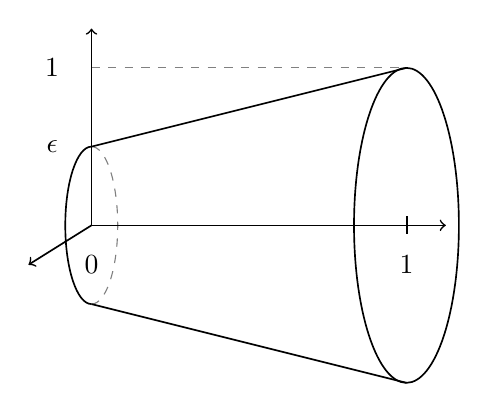
\begin{tikzpicture}
	\draw[dashed,color=gray] (0,-1) arc (-90:90:0.333 and 1);% right half of the left ellipse
	\draw[semithick] (4,-2) -- (0,-1);% bottom line
	\draw[semithick] (4,2) -- (0,1);% top line
	\draw[semithick] (0,-1) arc (270:90:0.333 and 1);% left half of the left ellipse
	\draw[semithick] (4,0) ellipse (0.666 and 2);% right ellipse
	\draw (-0.5,1) node {$\epsilon$};
  % x-Achse
	\draw[-,semithick] (0,0) -- (4,0);
	\draw[|->,semithick] (4,0) -- (4.5,0);
  % y-Tick
  \draw[dashed,color=gray] (0,2) -- (4,2);
  % y-Achse
  \draw[->,semithick] (0,0) -- (0,2.5);
  % z-Achse
  % TODO
  \draw[->,semithick] (0,0) -- (-0.8,-0.5);
	\draw (0,-0.5) node {$0$};
  \draw (-0.5,2) node {$1$};
	\draw (4,-0.5) node {$1$};
\end{tikzpicture}
\end{center}
We first calculate $V$ and $W$ from the given $f$ and then evaluate the
$x$-integral left in the formula of the error term:
\begin{equation}
  \begin{split}
    f(x) &:= x + \epsilon \\
    V(x) &= (x + \epsilon)^{-2} \\
    W(x) &= -\frac 2{V(x)}
  \end{split}
\end{equation}
The contributions at the boundaries can be read off immediately, since we don't
need to integrate there. At $x=0$ we have
\begin{equation}
  \label{res:boundary0}
  -\frac{5}{48}(2\log(2\epsilon^{-2}) - 1),
\end{equation}
at $x=1$ we get
\begin{equation}
  \label{res:boundary1}
  \frac{5}{48}(2\log(2(\epsilon + 1)^{-2}) -1).
\end{equation}
In the naive limit $\epsilon\to0$ we get the following contribution from the
boundary:
\begin{equation*}
  \frac{5}{48}(1-2\log(2))
\end{equation*}
The terms of the interior parametrix can be dealt with using the method
described in the main part of this section (or using a CAS) and we get the
following result for the error term (where the boundary contributions have
already been added):
\begin{align}
  &\frac{(\epsilon + 1)\log(\epsilon + 1)}{40}
  (\epsilon^4 + 4\epsilon^3 + 26\epsilon^2 + 44\epsilon + 26) \\
  &-
  \frac{\epsilon\log(\epsilon)}{40}
    \epsilon\log(\epsilon)(\epsilon^4 + 20\epsilon^2 + 5) \\
    &-
  \frac{\log(2)}{80}(5\epsilon^5 + 10\epsilon^3 + 70\epsilon^2 + 64\epsilon+26)
  \\
  &+ \frac{\epsilon(\epsilon+1)}{480}(13\epsilon^2 + 13\epsilon + 153)
  -\frac{193}{3600}.
\end{align}
For completeness' sake we evaluate again the naive limit $\epsilon\to0$ to be
\begin{equation}
  -\frac{13\log(2)}{40}-\frac{193}{3600} \approx -0.28.
\end{equation}
This result could be compared with a more careful approach to evaluate the error
term for a cone.
